\documentclass[serif,12pt]{beamer}
\usetheme{Copenhagen}
%\usecolortheme{dolphin}
\usepackage[utf8]{inputenc}
\usepackage[spanish]{babel}

\usepackage{multicol}

\usepackage{framed}
\usepackage{color}
\usepackage{wrapfig}\definecolor{shadecolor}{RGB}{224,238,238}



\begin{document}

\title[Integrating NoSQL in VO - Big Data challenges]{Integrating NoSQL into VO to support Big Data Challenges}  
\author[José Antonio Magro Cortés]{José Antonio Magro Cortés}
\institute[UGR]{TFM - Máster en Métodos y Técnicas Avanzadas en Física}
\date[Septiembre 2013]


%%%%%%%%%%%%%%%%%%%%%%%%%%%%%%%%%%%%%%%%%%%%%%%%%%%%%%%%%%%%%%%%%%%%%%%%%%%%%%%%%%%%%%%
% dia 1 - título
\begin{frame}
\titlepage
\end{frame}
%%%%%%%%%%%%%%%%%%%%%%%%%%%%%%%%%%%%%%%%%%%%%%%%%%%%%%%%%%%%%%%%%%%%%%%%%%%%%%%%%%%%%%%



%%%%%%%%%%%%%%%%%%%%%%%%%%%%%%%%%%%%%%%%%%%%%%%%%%%%%%%%%%%%%%%%%%%%%%%%%%%%%%%%%%%%%%%
% dia 2 - contenido
\begin{frame}
\frametitle{Contenido}
\scriptsize
\tableofcontents
\normalsize
\end{frame} 
%%%%%%%%%%%%%%%%%%%%%%%%%%%%%%%%%%%%%%%%%%%%%%%%%%%%%%%%%%%%%%%%%%%%%%%%%%%%%%%%%%%%%%%



%%%%%%%%%%%%%%%%%%%%%%%%%%%%%%%%%%%%%%%%%%%%%%%%%%%%%%%%%%%%%%%%%%%%%%%%%%%%%%%%%%%%%%%
% dia 3 - objetivo
\section{Objetivo}
\begin{frame}
\frametitle{Objetivo}


Realizar un estudio sobre la problemática de \emph{Big Data} en astronomía y proponer tecnologías alternativas a las existentes, dentro del Observatorio Virtual.


\end{frame}
%%%%%%%%%%%%%%%%%%%%%%%%%%%%%%%%%%%%%%%%%%%%%%%%%%%%%%%%%%%%%%%%%%%%%%%%%%%%%%%%%%%%%%%



%%%%%%%%%%%%%%%%%%%%%%%%%%%%%%%%%%%%%%%%%%%%%%%%%%%%%%%%%%%%%%%%%%%%%%%%%%%%%%%%%%%%%%%
% dia 4 - motivación
\section{Motivación}
\begin{frame}
\frametitle{Motivación}


\begin{itemize}
\item A raíz del curso \emph{Archivos Astronómicos: El Observartorio Virtual} (MTAF):
  \begin{itemize}
  \item Problemas en la gestión de grandes volúmenes de datos en el VO.
  \item Inadecuación de:
    \begin{itemize}
    \item DBMS.
    \item Formatos.
    \item Tecnologías.
    \end{itemize}
  \end{itemize}
\end{itemize}

\end{frame}
%%%%%%%%%%%%%%%%%%%%%%%%%%%%%%%%%%%%%%%%%%%%%%%%%%%%%%%%%%%%%%%%%%%%%%%%%%%%%%%%%%%%%%%


\section{Big Data}
%%%%%%%%%%%%%%%%%%%%%%%%%%%%%%%%%%%%%%%%%%%%%%%%%%%%%%%%%%%%%%%%%%%%%%%%%%%%%%%%%%%%%%%

%%%%%%%%%%%%%%%%%%%%%%%%%%%%%%%%%%%%%%%%%%%%%%%%%%%%%%%%%%%%%%%%%%%%%%%%%%%%%%%%%%%%%%%
% dia 5 - problema
\subsection{Definición}
\begin{frame}
\frametitle{Definición}

\textbf{big data} \emph{noun}: \footnote{10gen Big Data Whitepaper}

\begin{shaded}
%\emph{Conjuntos de datos tan grandes y complejos que dificultan su procesamiento mediante los sistemas actuales y tradicionales de gestión de bases de datos. Los problemas principales son la captura, clasificación, sistematización, almacenamiento, búsqueda, compartición, transferencia, análisis y visualización.}

referring to technologies and initiatives that
involve data that is too diverse, fast-changing or
massive for conventional technologies, skills and
infrastructure to address efficiently.


\end{shaded}
\end{frame}
%%%%%%%%%%%%%%%%%%%%%%%%%%%%%%%%%%%%%%%%%%%%%%%%%%%%%%%%%%%%%%%%%%%%%%%%%%%%%%%%%%%%%%%
% dia 6 - problema
\subsection{Problemas (I)}

\begin{frame}
\frametitle{Problemas (I)}

\begin{figure}
\centering
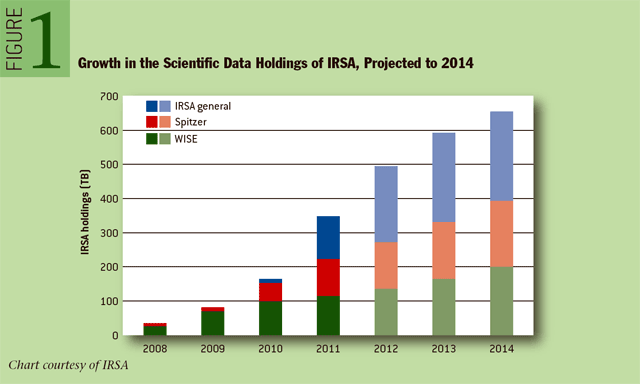
\includegraphics[width=0.7\textwidth, height=0.7\textheight]{images/data_rates.png} 
\label{fig:data_rates}
\end{figure}


\end{frame}
%%%%%%%%%%%%%%%%%%%%%%%%%%%%%%%%%%%%%%%%%%%%%%%%%%%%%%%%%%%%%%%%%%%%%%%%%%%%%%%%%%%%%%%
% dia 6 - problema
\subsection{Problemas (II)}

\begin{frame}
\frametitle{Problemas (II)}

\begin{itemize}
\item ALMA: 200 TB/año en el ALMA Archive
\item SKA: \emph{ultimate Big Data challenge}, 1 ExaFLOP/s
\item MWA: 3 PB/año
\item LSST: 30 TB/día
\end{itemize}


\end{frame}
%%%%%%%%%%%%%%%%%%%%%%%%%%%%%%%%%%%%%%%%%%%%%%%%%%%%%%%%%%%%%%%%%%%%%%%%%%%%%%%%%%%%%%%
% dia 6 - problema
\subsection{Problemas (III)}

\begin{frame}
\frametitle{Problemas (III)}

Bases de datos relacionales:\newline
\begin{itemize}
\item Ineficientes para el procesamiento distribuido.
\item Limitaciones en la velocidad de las consultas.
\item Falta de escalabilidad.
\end{itemize}


\end{frame}
%%%%%%%%%%%%%%%%%%%%%%%%%%%%%%%%%%%%%%%%%%%%%%%%%%%%%%%%%%%%%%%%%%%%%%%%%%%%%%%%%%%%%%%
% dia 6 - problema
\subsection{Solución}

\begin{frame}
\frametitle{Solución}

MongoDB: Base de datos NoSQL orientada a documentos.

\begin{figure}
\centering
\includegraphics[width=0.3\textwidth, height=0.3\textheight]{images/logo_mongodb.png} 
\label{fig:mongo_logo}
\end{figure}

\end{frame}
%%%%%%%%%%%%%%%%%%%%%%%%%%%%%%%%%%%%%%%%%%%%%%%%%%%%%%%%%%%%%%%%%%%%%%%%%%%%%%%%%%%%%%



\section{NoSQL}
%%%%%%%%%%%%%%%%%%%%%%%%%%%%%%%%%%%%%%%%%%%%%%%%%%%%%%%%%%%%%%%%%%%%%%%%%%%%%%%%%%%%%%%
\subsection{Definición}
\begin{frame}
\frametitle{Definición}

\begin{center}
NoSQL = \emph{Not Only SQL}
\end{center}

Tipos de BD NoSQL: orientadas a \textcolor{red}{documentos}, grafos, objetos, tabulares, etc.\newline


\begin{multicols}{2}

\textbf{Ventajas}
\begin{itemize}
\item Escalabilidad
\item Modelos de datos flexibles
\item Bajo coste
\end{itemize}

\textbf{Inconvenientes}
\begin{itemize}
\item Relativamente reciente
\item Soporte
\item Pocos usuarios
\end{itemize}

\end{multicols}

\end{frame}
%%%%%%%%%%%%%%%%%%%%%%%%%%%%%%%%%%%%%%%%%%%%%%%%%%%%%%%%%%%%%%%%%%%%%%%%%%%%%%%%%%%%%%%

\subsection{¿Qué es un documento?}
\begin{frame}
\frametitle{¿Qué es un documento?}

\begin{figure}
\centering
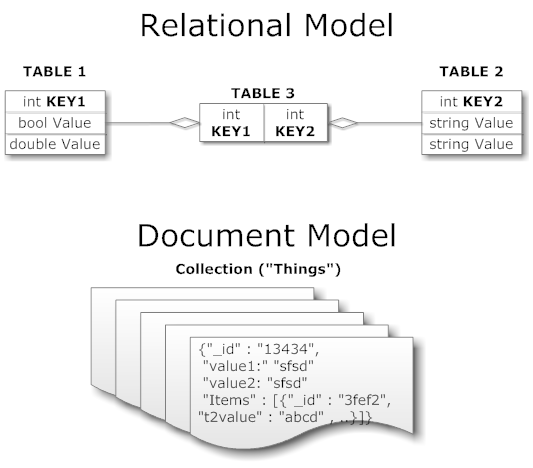
\includegraphics[width=0.6\textwidth, height=0.6\textheight]{images/document_vs_tables.png} 
\label{fig:document_vs_tables}
\end{figure}

\end{frame}

%%%%%%%%%%%%%%%%%%%%%%%%%%%%%%%%%%%%%%%%%%%%%%%%%%%%%%%%%%%%%%%%%%%%%%%%%%%%%%%%%%%%%%%
\subsection{MongoDB}
\begin{frame}
\frametitle{MongoDB}

\begin{itemize}
\item Orientada a documentos
\item Drivers para varios lenguajes
\item Soporte completo para índices
\item Fácil instalación y puesta en marcha
\item Balanceo de carga
\item Soporta MapReduce
\item Conexión con Hadoop
\item Tecnología actual para problemas actuales
\end{itemize}

\end{frame}
%%%%%%%%%%%%%%%%%%%%%%%%%%%%%%%%%%%%%%%%%%%%%%%%%%%%%%%%%%%%%%%%%%%%%%%%%%%%%%%%%%%%%%%

\subsection{Casos de éxito}
\begin{frame}
\frametitle{Casos de éxito}

\begin{itemize}
\item CMS en el LHC: 10 PB de datos cada año.
\item ATLAS Workload Management System.
\item Medida de niveles de radiación en Seattle.
\item Mars Science Lab para comunicación con rovers.
\end{itemize}


\end{frame}
%%%%%%%%%%%%%%%%%%%%%%%%%%%%%%%%%%%%%%%%%%%%%%%%%%%%%%%%%%%%%%%%%%%%%%%%%%%%%%%%%%%%%%%





%%%%%%%%%%%%%%%%%%%%%%%%%%%%%%%%%%%%%%%%%%%%%%%%%%%%%%%%%%%%%%%%%%%%%%%%%%%%%%%%%%%%%%%
\section{NoSQL en el VO}


\subsection{Problemas en el VO}
\begin{frame}
\frametitle{Problemas en el VO}

\begin{itemize}
\item FITS
  \begin{itemize}
    \item Almacenamiento en archivos.
    \item Varias convenciones: IDI, SD, MB, OI.
    \item Múltiples combinaciones clave-valor.
  \end{itemize}
\item TAP/OpenCADC: sólo lenguajes relacionales (ADQL/PQL).
\end{itemize}

\end{frame}



%%%%%%%%%%%%%%%%%%%%%%%%%%%%%%%%%%%%%%%%%%%%%%%%%%%%%%%%%%%%%%%%%%%%%%%%%%%%%%%%%%%%%%%
\subsection{Solución: NoSQL en el VO}
\begin{frame}
\frametitle{Solución: NoSQL en el VO}

\begin{itemize}
\item Almacén FITS en documentos MongoDB.
\item Conexión OpenCADC y NoSQL para ALMA: Java y driver MongoDB.
\end{itemize}


\end{frame}
%%%%%%%%%%%%%%%%%%%%%%%%%%%%%%%%%%%%%%%%%%%%%%%%%%%%%%%%%%%%%%%%%%%%%%%%%%%%%%%%%%%%%%%


%%%%%%%%%%%%%%%%%%%%%%%%%%%%%%%%%%%%%%%%%%%%%%%%%%%%%%%%%%%%%%%%%%%%%%%%%%%%%%%%%%%%%%%
\section{Conclusiones y trabajo futuro}
\begin{frame}
\frametitle{Conclusiones y trabajo futuro}

\begin{multicols}{2}

\textbf{Conclusiones}
\begin{itemize}
\item NoSQL más eficiente para algunos problemas
\item Menor coste para análisis y diseño
\item Facilidad para incorporar frameworks de VO a NoSQL
\end{itemize}

\textbf{Trabajo futuro}
\begin{itemize}
\item Adaptar OpenCADC a NoSQL
\item Usar métricas formales de diseño
\item Benchmarks para medir rendimiento
\end{itemize}

\end{multicols}

\end{frame}
%%%%%%%%%%%%%%%%%%%%%%%%%%%%%%%%%%%%%%%%%%%%%%%%%%%%%%%%%%%%%%%%%%%%%%%%%%%%%%%%%%%%%%%

\end{document}
